\section{Asymetrické šifry}
Asymetrickou šifrou se rozumí taková šifra, u které klíč pro dešifrování nelze výpočetně snadno získat z klíče pro zašifrování. Též se používá pojem šifra s veřejným klíčem jelikož jeden z vygenerovaných klíčů oprávněných stran, může být navíc veřejně dostupný \parencite{tesar2021}.

Asymetrickou šifrou lze také řešit problém ověření autora identity účastníků komunikace. Mohli bychom si představit situaci, kdy Alice chce poslat Bobovi šifrovanou zprávu a Bob si mohl být si jistý, že zpráva skutečně pochází od ní. Alice a Bob si vygenerují své páry soukromých a veřejných klíčů. Alice zašifruje zprávu svým soukromým klíčem (pro digitální podpis) a následně ji zašifruje Bobovým veřejným klíčem. Bob zprávu dešifruje svým soukromým klíčem a ověří autenticitu zprávy použitím veřejného klíče \parencite{burda2019}.

Tímto způsobem asymetrická kryptografie zajišťuje autenticitu odesílatele, integritu zprávy a důvěrnost komunikace. Typickým příkladem je právě šifra RSA.

\subsection{Šifra RSA}
RSA \enquote{(Rivest-Shamir-Adleman)} je jednou z nejznámějších asymetrických šifer. Tento algoritmus, vyvinutý na základě myšlenky veřejného klíče, je inspirací inspirovanou prací Diffieho a Hellmana \parencite{diffie1976} a byl plně realizován v práci \textcite{rsa1978}. RSA umožňuje nejen šifrování dat, ale také digitální podepisování, což zajišťuje autentizaci a integritu informací.

Dle \textcite{rsa1978} je základem RSA algoritmu následující postup:

\begin{enumerate}
    \item \textbf{Generování klíčů:}
      \begin{itemize}
        \item Vyberte dvě velká prvočísla \( p \) a \( q \).
        \item Vypočítejte modul \( n = p \cdot q \), který slouží jako základ pro oba klíče.
        \item Spočtěte Eulerovu funkci \(\varphi(n) = (p-1)(q-1)\).
      \end{itemize}
  
    \item \textbf{Volba veřejného klíče:}
      \begin{itemize}
        \item Zvolte celé číslo \( e \) tak, aby \( 1 < e < \varphi(n) \) a \( e \) bylo nesoudělné s \(\varphi(n)\). Číslo \( e \) slouží jako veřejný exponent.
      \end{itemize}
    
    \item \textbf{Výpočet soukromého klíče:}
      \begin{itemize}
        \item Určete číslo \( d \), které je multiplikativní inverzí \( e \) modulo \(\varphi(n)\), tedy splňuje rovnici:
        \[
        e \cdot d \equiv 1 \pmod{\varphi(n)}.
        \]
        Číslo \( d \) je soukromým exponentem.
      \end{itemize}
    
    \item \textbf{Šifrování a dešifrování:}
      \begin{itemize}
        \item Veřejný klíč je tvořen dvojicí \((n, e)\) a soukromý klíč dvojicí \((n, d)\).
        \item Pro šifrování zprávy \( m \) (kde \( m < n \)) se vypočítá šifrovaná zpráva:
        \[
        c = m^e \mod n.
        \]
        \item Pro dešifrování se použije:
        \[
        m = c^d \mod n.
        \]
      \end{itemize}
  \end{enumerate}

Přestože veřejný klíč \((n, e)\) je znám, bez znalosti velkých prvočísel \( p \) a \( q \) (délky alespoň 2048 bitů), je výpočetně velmi složité získat soukromý klíč \((n, d)\). Tento bezpečnostní předpoklad vychází z faktu, že faktorizace čísla \( n \) na jeho prvočinitele je výpočetně velmi náročný úkol - tzv. NP-těžký problém, který má exponenciální složitost pro klasické výpočetní prostředky \parencite{tesar2021}.  

\label{sec:asymetricka-kryptografie}
Jedním z nejvýznamnějších využití tohoto kryptografického protokolu jsou digitální podpisy, které umožňují ověřovat jak autentifikaci, tak i integritu dat. V tomto procesu soukromý klíč slouží k podepsání zprávy, čímž garantuje její původ a nezaměnitelnost, zatímco veřejný klíč příjemci umožňuje ověřit, že zpráva pochází od oprávněného odesílatele a nebyla nijak pozměněna během přenosu třetí stranou.

V oblasti bezpečnosti internetových připojení nachází asymetrická kryptografie své praktické využití zejména v protokolech SSL a TLS, které slouží k vytváření bezpečného spojení mezi klientem a serverem. Během navazování spojení (tzv. handshake) asymetrické šifrování umožňuje autentifikaci serveru a bezpečnou výměnu symetrického klíče. Tento symetrický klíč je následně použít k šifrování přenášených dat již většího objemu \parencite{wikijs2024}. Pro výměnu příslušných klíčů je často využívána, díky její rychlosti, metoda Diffie-Hellman, jež byla popsána v předchozí kapitole.

Dalším významným využitím asymetrické kryptografie je v případě elektronické měny Bitcoin. V bitcoinu, používáme kryptografii pro vytvoření páru klíčů, které kontrolují přístup k bitcoinům. Tento pár klíčů se skládá ze soukromého klíče a z něho odvozeného jedinečného veřejného klíče. Veřejný klíč je použit pro příjem bitcoinů a soukromý klíč je použit pro podpis transakce, která tyto bitcoiny utrácí \parencite{antonopoulos2014}.

\enquote{Při utrácení bitcoinů, současný vlastník bitcoinů poskytuje jeho veřejný klíč a podpis (pokaždé různý, ale vytvořený ze stejného soukromého klíče) transakce, aby mohl utratit tyto bitcoiny. Po poskytnutí veřejného klíče a podpisu, každý v bitcoinové síti může ověřit a přijmout transakci jako platnou, potvrdit, že osoba převádějící bitcoiny je vlastní v okamžiku převodu} \parencite{antonopoulos2014}.

Asymetrická kryptografie hraje tedy významnou roli v vytváření klíčů a podepisování transakcí. Nutno podotknout, že ze znalosti veřejného klíče, je výpočetně složité nalézt klíč privátní. Tento typ asymetrické kryptografie je založena na problému diskrétního logaritmu vyjádřeného sčítáním a násobením bodů na eliptické křivce \parencite{antonopoulos2014}.

Nevýhodou asymetrické kryptografie může být nižší rychlost šifrování oproti symetrickým šifrám, což ji činí nevhodnou pro přímé šifrování velkých bloků dat. Proto se asymetrická kryptografie často využívá v kombinaci se symetrickou, například při výměně klíčů v hybridních šifrovacích systémech.

V praxi se tak nejčastěji můžeme setkat s kombinací algoritmů ECDSA nebo EDDSA, který používají pro generování klíče Eliptické křivky (EC). Šifra DSA se od RSA prakticky neliší, pouze používá problém diskrétního logaritmu (viz. \hyperref[sec:diffie-hellman]{Diffie-Helmannův protokol}) k generování páru klíčů. Ve výsledku je rozdíl mezi těmito algoritmy v rychlosti, nikoli v bezpečnosti. Funkčně, kde RSA a DSA vyžadují klíče velikosti 3072 bitů k dosažení požadované úrovně bezpečnosti, ECDSA toho dosahuje pouze s klíči o délce 256-bitů \parencite{kontsevoy2020}.

\begin{figure}[htbp]
    \centering
    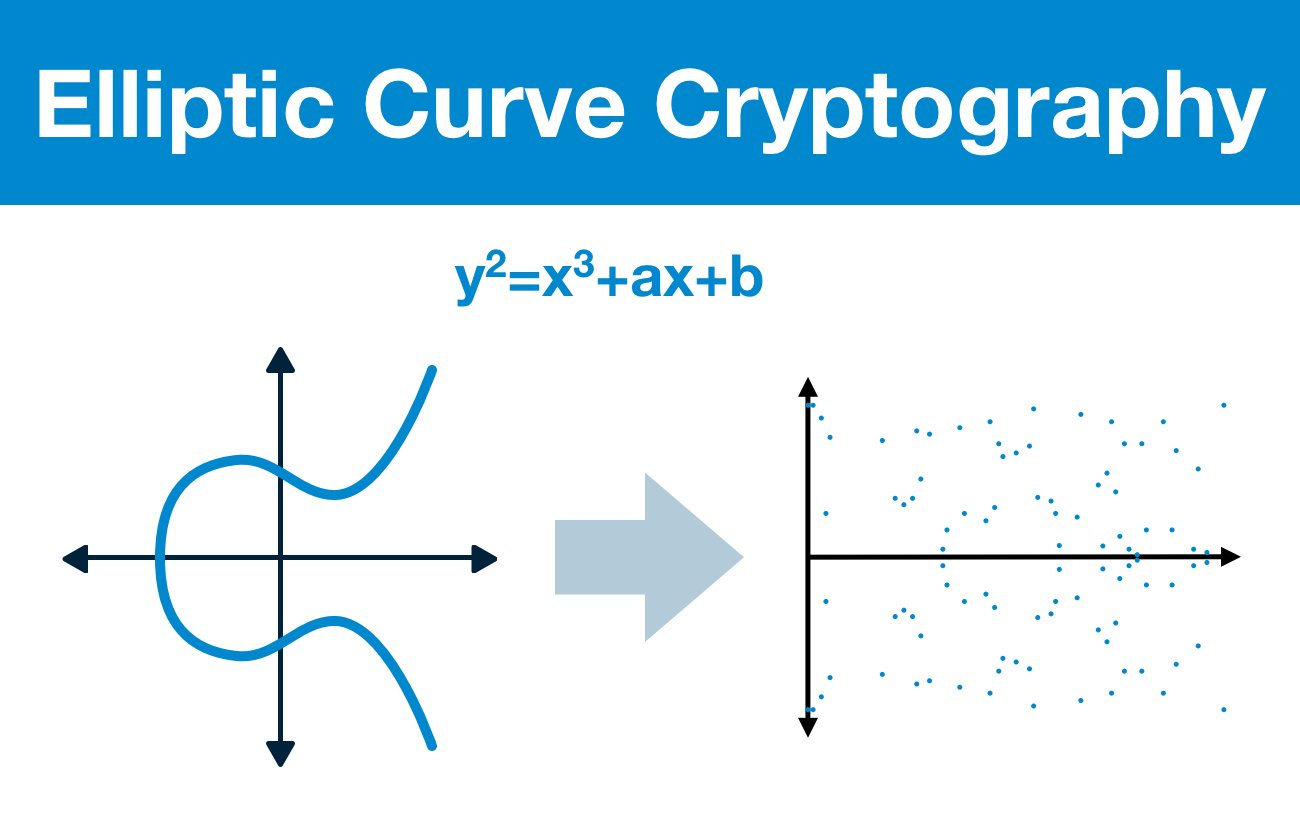
\includegraphics[width=1\textwidth]{\FIGURES/elliptic-curve-cryptography-1.jpeg}
    \caption{Eliptická křivka znázorněna matematickou funkcí. Zdroj: \parencite{eliptic-curve-1}}
    \label{fig:elliptic-curve-cryptography}
  \end{figure}
\newpage